
\documentclass{iacrtrans}
\makeatletter
\renewcommand{\addcontentsline}[3]{}
\makeatother
\usepackage{amsmath}
\usepackage{amsfonts}
\usepackage{amssymb}
\usepackage{booktabs}
\usepackage{stmaryrd}
\usepackage{graphicx}
\usepackage{tikz}
\usetikzlibrary{positioning,arrows.meta}

\usepackage{listings}
\usepackage{caption}
\usepackage{subcaption}
\usepackage{mathpartir}
\usepackage{syntax}
\usepackage{comment}
\usepackage{verbatim}
\usepackage{url}

\title{Graded Typing}
\author{Elazar Gershuni}
\date{Sept 2025}

\begin{document}

\maketitle

\newcommand{\Var}{\mathsf{Var}}
\newcommand{\Any}{\mathsf{Any}}
\newcommand{\Int}{\mathsf{Int}}
\newcommand{\String}{\mathsf{String}}
\newcommand{\Bool}{\mathsf{Bool}}
\newcommand{\rank}{\mathsf{rank}}
\newcommand{\raiseTo}[1]{\uparrow^{#1}}
\newcommand{\ceil}[1]{\left\lceil #1 \right\rceil}

\begin{abstract}
Path-insensitive analyses are efficient but collapse precision at control-flow joins, merging distinct types into a single ``unknown.'' 
We make this loss explicit and quantifiable by introducing a \emph{graded} algebra of types. 
Base types and $\Any$ carry a nonnegative grade $i$, written $X^{i}$ and $\Any^{i}$. 
Grades increase only when an imprecise value is \emph{coerced to a base}, via the step $\Any^{i} \le X^{\,i+1}$; heterogeneous joins are conservative, yielding $\Any^{r}$ at a common grade $r$ when $X\neq Y$. 
Thus every type carries a record of \emph{how many assumptions} have been made about it, and these increments can be attributed to specific program sites.

We instantiate this graded domain in a standard abstract interpreter for a while-language. 
Transfer functions are monotone; joins are associative, commutative, and idempotent. 
Although the global lattice has infinite height, each program inhabits a finite slice, since grades can increase only at finitely many sites. 
Fixed-point iteration therefore converges without widening. 
The analysis is a sound may-analysis: it does not eliminate runtime type errors, but it records and localizes imprecision. 
A lightweight ghost-state instrumentation yields \emph{bounded blame}: any runtime type fault can be traced to a small, computed set of program sites.

Conceptually, this is an ``unfolded'' view of gradual typing. 
Standard gradual typing is recovered by collapsing grades ($X^{i}\mapsto X$, $\Any^{i}\mapsto ?$) and reintroducing consistency and casts. 
We also sketch conservative extensions (grade-parametric function signatures, graded effects, SSA $\phi$-site instrumentation) that reuse the same algebra. 
The core requires no language changes and no runtime checks.
\end{abstract}

\section{Introduction}

Path-insensitive analyses are fast and predictable, but they routinely \emph{collapse} information at control-flow joins.
A common outcome is that a variable alternately assigned an integer and a string is reported as a single top-like ``unknown,'' and every downstream use inherits that imprecision.
The analysis remains sound as an over-approximation, but it is hard to act on: we learn \emph{that} precision was lost, not \emph{where} or \emph{how much}.

We propose an \emph{unfolded} view of the unknown: a ranked algebra of types that makes loss of precision explicit and compositional.
Base types (\(\mathsf{Int},\mathsf{String},\mathsf{Bool}\)) and \(\mathsf{Any}\) are annotated with a nonnegative \emph{rank} \(i\), written \(X^{i}\) and \(\mathsf{Any}^{i}\).
Joins are conservative: after promotion to a common rank \(r\), merging incompatible bases at that rank yields \(\mathsf{Any}^{r}\) (no bump).
Ranks increase only when the analysis \emph{commits to a base after imprecision}:
the subtyping step \(\mathsf{Any}^{i} \le X^{\,i+1}\) captures the ``downcast'' (assumption) that reinterprets an imprecise value as a concrete base, and increments the rank.
Operational semantics are unchanged; ranks live purely in the analysis.

Two consequences follow.
First, ranked types record—at the right granularity—\emph{how much} imprecision was assumed and (via site IDs) \emph{where} assumptions were forced.
Second, although the global order has infinite height, each program inhabits a finite slice:
rank can go up only where a base is demanded after a loss of correlation, and each site is idempotent in the abstract interpretation.
A standard fixed-point computation therefore converges \emph{without} bespoke widenings.

\paragraph{Unfolded gradual typing.}
Conceptually, this is an \emph{unfolded} form of gradual typing: instead of a single unknown \(?\), we expose a stratified family \(\mathsf{Any}^{0},\mathsf{Any}^{1},\ldots\) that records how many assumptions were needed.
Standard gradual typing is recovered by \emph{collapsing} ranks (erasing \(X^{i}\mapsto X\), \(\mathsf{Any}^{i}\mapsto ?\)) and adding the usual consistency/cast machinery.
We keep the core static and cast-free; a small extension adds rank-aware casts and a collapsed, consistency-based mode.

\paragraph{Contributions.}
\begin{itemize}
  \item A minimal ranked type algebra that exposes path-insensitive precision loss as an integer index on types. Joins promote to a common rank and return \(\mathsf{Any}^{r}\) for heterogeneous bases; ranks increase only at \emph{downcasts} \(\mathsf{Any}^{i}\le X^{\,i+1}\).
  \item A conventional abstract interpreter for a while-language over this domain, with monotone transfer functions and per-program convergence \emph{without} widening (per-site idempotence).
  \item Properties and diagnostics: per-program finiteness; a bounded-blame principle via ghost culprit sets that localizes assumptions to a small set of program sites; and a clear account of what the analysis guarantees (and does not).
\end{itemize}

\paragraph{Utility.}
The immediate use case is diagnostic: instead of reporting a bare ``\(\mathsf{Any}\),'' the analyzer reports \(\mathsf{Any}^{k}\) and points to the joins/uses that forced \(k\) assumptions.
Because rank growth is tied to identifiable choke points where a base is demanded, remediation focuses on a bounded set of locations.
The scheme is unobtrusive: no runtime checks, no language changes, and no change to concrete semantics.


\section{The \textsf{Graded} Type System}
\label{sec:types}

We factor path-insensitivity at control-flow joins into a lightweight, \emph{grade}-annotated type algebra. Grades are \emph{static} metadata; runtime values are unannotated. Intuitively, a grade increases exactly when the analysis must \emph{commit to a base after imprecision}; i.e., when downcasting from $\Any$ to a concrete base via subtyping. Heterogeneous joins themselves do not raise the grade.

\paragraph{Indices and intuition.}
Grades range over $\mathbb{N}=\{0,1,2,\dots\}$, with two distinguished symbols:
a formal bottom $\bot$ used only by $\Any^{\bot}$, and an absorbing top $\infty$ used only by $\Any^{\infty}$.
Base literals appear at grade $0$.
We extend $\max$ by $\max(\bot,j)=j$ for $j\in\mathbb{N}$ (and never apply $+1$ to $\bot$ or $\infty$).

\begin{figure}[t]
\centering
\[
\begin{array}{rcll}
i &::=& 0 \mid 1 \mid 2 \mid \cdots & \text{(finite grades)}\\[2pt]
X &::=& \Int \mid \String \mid \Bool & \text{(base types)}\\[2pt]
\tau &::=& X^{i} \mid \Any^{i} \mid \Any^{\bot} \mid \Any^{\infty} & \text{(graded types)}
\end{array}
\]
\vspace{-2mm}
\caption{Syntax of graded types.}
\label{fig:syntax}
\end{figure}

\begin{figure}[ht]
\centering
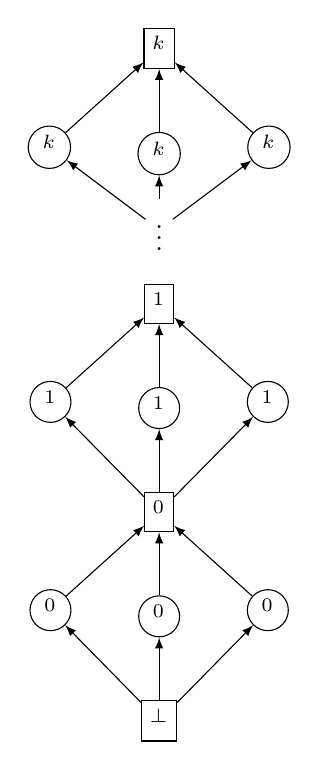
\begin{tikzpicture}[
    node distance=0.8cm and 1cm,
    base/.style={circle, draw, inner sep=2pt},
    any/.style={rectangle, draw, inner sep=3pt}
]
    % Grade k (Top)
    \node (anyk) [any] {$\Any^k$};
    \node (intk) [base, below left=of anyk] {$\Int^k$};
    \node (strk) [base, below=of anyk] {$\String^k$};
    \node (boolk) [base, below right=of anyk] {$\Bool^k$};
    
    \draw[-latex] (intk) -- (anyk);
    \draw[-latex] (strk) -- (anyk);
    \draw[-latex] (boolk) -- (anyk);

    % Ellipsis
    \node (vdots) [below=of strk, yshift=0.5cm] {\vdots};

    % Grade 1
    \node (any1) [any, below=of vdots, yshift=0.5cm] {$\Any^1$};
    \node (int1) [base, below left=of any1] {$\Int^1$};
    \node (str1) [base, below=of any1] {$\String^1$};
    \node (bool1) [base, below right=of any1] {$\Bool^1$};

    \draw[-latex] (int1) -- (any1);
    \draw[-latex] (str1) -- (any1);
    \draw[-latex] (bool1) -- (any1);
    
    % Connections from rank k-1 to k
    \path (vdots) edge[-latex] (intk);
    \path (vdots) edge[-latex] (strk);
    \path (vdots) edge[-latex] (boolk);

    % Grade 0
    \node (any0) [any, below=of str1] {$\Any^0$};
    \node (int0) [base, below left=of any0] {$\Int^0$};
    \node (str0) [base, below=of any0] {$\String^0$};
    \node (bool0) [base, below right=of any0] {$\Bool^0$};

    \draw[-latex] (int0) -- (any0);
    \draw[-latex] (str0) -- (any0);
    \draw[-latex] (bool0) -- (any0);
    
    % Connections from rank 0 to 1
    \draw[-latex] (any0) -- (int1);
    \draw[-latex] (any0) -- (str1);
    \draw[-latex] (any0) -- (bool1);
    
    \node (anybot) [any, below=of str0] {$\Any^{\bot}$};
    
    \draw[-latex] (anybot) -- (int0);
    \draw[-latex] (anybot) -- (str0);
    \draw[-latex] (anybot) -- (bool0);
\end{tikzpicture}
\caption[Hasse diagram of the graded type lattice]%
{Hasse diagram of the graded type lattice. Each rank $i$ consists of base types below $\Any^i$. 
The ranks are connected by the subtyping rule $\Any^i \le X^{i+1}$, forming a vertical chain.}
\label{fig:hassediagram}
\end{figure}

\paragraph{Subtyping.}
Subtyping is the least reflexive–transitive relation generated by the rules in Fig.~\ref{fig:subtyping}. Intuitively, $\Any^{i}$ is the bottom of grade $i$; moving from grade $i$ to $i{+}1$ reflects a \emph{downcast assumption} to a concrete base; $\Any^{\infty}$ is an absorbing top; and $\Any^{\bot}$ seeds grade~$0$.

\begin{figure}[t]
\centering
\begin{mathpar}
\inferrule*[right=(grade)]
  { }
  { X^{i} \;\le\; \Any^{i} }\quad(i\in\mathbb{N})
\qquad
\inferrule*[right=(Step)]
  { }
  { \Any^{i} \;\le\; X^{i+1} }\quad(i\in\mathbb{N})
\end{mathpar}
\vspace{-3mm}
\caption{Generating rules for subtyping ($X\in\{\Int,\String,\Bool\}$).}
\label{fig:subtyping}
\end{figure}

\paragraph{Join (\texorpdfstring{$\sqcup$}{sqcup}).}
$\sqcup$ is the least upper bound w.r.t.\ $\le$.
Its definition proceeds by \emph{promotion to a common grade} followed by a same-grade join (Fig.~\ref{fig:join}).

\begin{figure}[t]
\centering
\textbf{Promotion to common grade.}
Define $\grade(\Any^{\bot}){=}\bot$, $\grade(\Any^{i}){=}i$, $\grade(X^{i}){=}i$, $\grade(\Any^{\infty}){=}\infty$.
For $\tau_1,\tau_2$ with finite grades or $\bot$, set $r=\max(\grade(\tau_1),\grade(\tau_2))$ and let
\[
\uparrow^{r}(\tau) \;=\;
\begin{cases}
\tau & \text{if } \grade(\tau)=r,\\
\Any^{r} & \text{if } \grade(\tau)<r\text{ (promote to least supertype at grade $r$).}
\end{cases}
\]
(If any operand is $\Any^{\infty}$, the join is $\Any^{\infty}$.)

\medskip
\textbf{Same-grade join (at grade $r\in\mathbb{N}$).}
For $X,Y\in\{\Int,\String,\Bool\}$ and $Z\in\{\Any,\Int,\String,\Bool\}$:
\[
\begin{array}{r@{\quad=\quad}l@{\qquad}l}
X^{r} \sqcup X^{r} & X^{r} & \text{(idempotence)}\\
X^{r} \sqcup Y^{r} & \Any^{r} & (X\neq Y)\ \text{(heterogeneous merge; no bump)}\\
\Any^{r} \sqcup Z^{r} & \Any^{r} & \text{(absorption)}\\
\end{array}
\]
\medskip
\textbf{Full definition.}
\[
\tau_1 \sqcup \tau_2 \;=\;
\begin{cases}
\Any^{\infty} & \text{if }\tau_1=\Any^{\infty}\text{ or }\tau_2=\Any^{\infty},\\
\uparrow^{r}(\tau_1)\ \sqcup\ \uparrow^{r}(\tau_2) & \text{where } r=\max(\grade(\tau_1),\grade(\tau_2)).
\end{cases}
\]
\vspace{-1mm}
\caption{Join: promote to a common grade, then same-grade join.}
\label{fig:join}
\end{figure}

\paragraph{Derived laws.}
For all $i\le j$ in $\mathbb{N}$ and $X\in\{\Int,\String,\Bool\}$:
\begin{align*}
&\textbf{Monotone grades:} && \Any^{i} \le \Any^{j},\quad X^{i} \le X^{j}.\\
&\textbf{Absorption (same grade):} && \Any^{i} \sqcup \tau^{i} = \Any^{i}.\\
&\textbf{Cross-grade absorption:} && \Any^{i} \sqcup \tau^{j} = \Any^{\max(i,j)}\quad(\text{with }\max(\bot,j)=j).\\
&\textbf{Heterogeneous same-grade merge:} && X^{i} \sqcup Y^{i}=\Any^{i}\ (X\neq Y).\\
&\textbf{Top absorption:} && \tau \sqcup \Any^{\infty}=\Any^{\infty}.\\
&\textbf{ACI of join:} && \text{$\sqcup$ is associative, commutative, idempotent.}
\end{align*}

\paragraph{Reading grades.}
With $\Any^{\bot}$ as a formal bottom, a finite grade $k\ge 0$ records the number of \emph{downcast assumptions} (steps of $\Any^{i}\le X^{i+1}$) witnessed so far along the abstract flow.
Once at $\Any^{k}$, further joins at grade $\le k$ do not escalate the grade; escalation requires a new downcast at or above grade $k$.
By convention, $\Any^{0}$ denotes imprecision \emph{without any forced assumption yet}:
merging heterogeneous bases at a join yields $\Any^{0}$ (after promotion), but grades increase only when a base is \emph{demanded} and a downcast $\Any^{i}\le X^{i+1}$ is taken.
Thus joins alone do not raise grades; uses that require a base do.

\medskip
This section defines only the graded type algebra.
The language and its abstract interpreter (expressions, statements, \textsf{while}) appear in the next section.

\section{Language and Abstract Interpretation}
\label{sec:lang-ai}

We use a standard \textsf{while}-language with integers, strings, and booleans. Runtime semantics are conventional and ungraded; grades appear only in the abstract domain of \S\ref{sec:types}.

\subsection{Syntax and Concrete Semantics}

\begin{figure}[t]
\centering
\[
\begin{array}{rcll}
v &::=& n \in \mathbb{Z} \;\mid\; s \in \Sigma^* \;\mid\; \mathsf{true} \;\mid\; \mathsf{false} & \text{(values)}\\[1pt]
e &::=& v \;\mid\; x \;\mid\; e{+}e \;\mid\; \neg e \;\mid\; e \wedge e \;\mid\; e {=} e & \text{(expressions)}\\[1pt]
s &::=& \mathsf{skip} \;\mid\; x {:=} e \;\mid\; s; s \;\mid\; \mathsf{if}\; e\;\mathsf{then}\; s\;\mathsf{else}\; s \;\mid\; \mathsf{while}\; e\;\mathsf{do}\; s & \text{(statements)}
\end{array}
\]
\vspace{-2mm}
\caption{Syntax of the \textsf{while}-language.}
\label{fig:syntax-while}
\end{figure}

A \emph{state} is a total map $\sigma: \Var \to (\mathbb{Z}\cup\Sigma^*\cup\{\mathsf{true},\mathsf{false}\})$.
We write $\langle e,\sigma\rangle \Downarrow v$ for big-step expression evaluation and
$\langle s,\sigma\rangle \Downarrow \sigma'$ for statement evaluation. The rules are standard and deterministic:
(i) $x$ looks up $\sigma(x)$; (ii) $+$ denotes integer addition on integers and string concatenation on strings;
(iii) $\neg,\wedge$ operate on booleans; (iv) $=$ compares values for equality and yields a boolean; (v) assignments update the state; (vi) sequencing, conditional, and while follow the textbook rules, with $\mathsf{while}\;e\;\mathsf{do}\;s$ defined via the usual unrolling into an \textsf{if}.
We omit the routine rule schemata for space.

\subsection{Abstract Interpretation}

We interpret programs over the graded type lattice of \S\ref{sec:types}.
An \emph{abstract environment} is a map $\Gamma:\Var\to\tau$.
Ordering and joins on environments are pointwise, using the subtyping $\le$ and join $\sqcup$ on types defined previously.

\paragraph{Grade-aware coercion to a base.}
For $X\in\{\Int,\String,\Bool\}$ and a type $\tau$, define the \emph{least $X$-supertype} by
\[
\ceil{\tau}_X \;=\; \min\nolimits_{\le}\,\{\,X^{k}\mid \tau \le X^{k}\,\}.
\]
Under the subtyping rules of Fig.~\ref{fig:subtyping}, $\ceil{\tau}_X$ always exists and is unique; intuitively, $\ceil{\cdot}_X$ “raises” $\tau$ to the nearest $X$-typed supertype (performing a downcast $\Any^{i}\!\le\!X^{i+1}$ exactly when needed).

\paragraph{Abstract expressions.}
We write $\Gamma \vdash e : \tau$ for abstract evaluation.

\begin{mathpar}
\inferrule*[right=(Lit)]
  { }
  { \Gamma \vdash n : \Int^{0} \qquad
    \Gamma \vdash s : \String^{0} \qquad
    \Gamma \vdash \mathsf{true} : \Bool^{0} \qquad
    \Gamma \vdash \mathsf{false} : \Bool^{0} }

\inferrule*[right=(Var)]
  { \Gamma(x)=\tau }
  { \Gamma \vdash x : \tau }

\inferrule*[right=(Sub)]
  { \Gamma \vdash e : \tau \quad \tau \le \tau' }
  { \Gamma \vdash e : \tau' }
\end{mathpar}

\noindent Operators coerce operands to the relevant base(s) using $\ceil{\cdot}_X$ and then combine grades via $\max$; when multiple operator interpretations apply, we join the results:

\begin{mathpar}
\inferrule*[right=(Plus$_\Int$)]
  { \Gamma \vdash e_1:\tau_1 \quad \Gamma \vdash e_2:\tau_2 \\
    \ceil{\tau_1}_\Int = \Int^{i} \quad \ceil{\tau_2}_\Int = \Int^{j} }
  { \Gamma \vdash e_1{+}e_2 : \Int^{\max(i,j)} }

\inferrule*[right=(Plus$_\String$)]
  { \Gamma \vdash e_1:\tau_1 \quad \Gamma \vdash e_2:\tau_2 \\
    \ceil{\tau_1}_\String = \String^{i} \quad \ceil{\tau_2}_\String = \String^{j} }
  { \Gamma \vdash e_1{+}e_2 : \String^{\max(i,j)} }

\inferrule*[right=(Plus-Join)]
  { \Gamma \vdash e_1{+}e_2 : \tau_I \quad \Gamma \vdash e_1{+}e_2 : \tau_S }
  { \Gamma \vdash e_1{+}e_2 : \tau_I \sqcup \tau_S }
\end{mathpar}

\begin{mathpar}
\inferrule*[right=(Not)]
  { \Gamma \vdash e:\tau \quad \ceil{\tau}_\Bool=\Bool^{i} }
  { \Gamma \vdash \neg e : \Bool^{i} }
\qquad
\inferrule*[right=(And)]
  { \Gamma \vdash e_1:\tau_1 \quad \Gamma \vdash e_2:\tau_2 \\
    \ceil{\tau_1}_\Bool=\Bool^{i} \quad \ceil{\tau_2}_\Bool=\Bool^{j} }
  { \Gamma \vdash e_1 \wedge e_2 : \Bool^{\max(i,j)} }
\end{mathpar}

\begin{mathpar}
\inferrule*[right=(Eq$_X$)]
  { X\in\{\Int,\String,\Bool\} \\
    \Gamma \vdash e_1:\tau_1 \quad \Gamma \vdash e_2:\tau_2 \\
    \ceil{\tau_1}_X = X^{i} \quad \ceil{\tau_2}_X = X^{j} }
  { \Gamma \vdash e_1 {=} e_2 : \Bool^{\max(i,j)} }
\\
\inferrule*[right=(Eq-Join)]
  { \Gamma \vdash e_1{=}e_2 : \rho_1 \quad
    \Gamma \vdash e_1{=}e_2 : \rho_2 }
  { \Gamma \vdash e_1{=}e_2 : \rho_1 \sqcup \rho_2 }
\end{mathpar}

\paragraph{Abstract statements.}
We write $\Gamma \vdash s \triangleright \Gamma'$ for the abstract transformer.

\begin{mathpar}
\inferrule*[right=(Skip)]
  { }
  { \Gamma \vdash \mathsf{skip} \triangleright \Gamma }

\inferrule*[right=(Assign)]
  { \Gamma \vdash e : \tau }
  { \Gamma \vdash x {:=} e \triangleright \Gamma[x \mapsto \tau] }

\inferrule*[right=(Seq)]
  { \Gamma \vdash s_1 \triangleright \Gamma_1 \quad
    \Gamma_1 \vdash s_2 \triangleright \Gamma_2 }
  { \Gamma \vdash s_1; s_2 \triangleright \Gamma_2 }

\inferrule*[right=(If)]
  { \Gamma \vdash e : \tau \quad \ceil{\tau}_\Bool=\Bool^{i} \\
    \Gamma \vdash s_1 \triangleright \Gamma_1 \quad
    \Gamma \vdash s_2 \triangleright \Gamma_2 }
  { \Gamma \vdash \mathsf{if}\; e\;\mathsf{then}\; s_1\;\mathsf{else}\; s_2
      \triangleright (\Gamma_1 \sqcup \Gamma_2) }
\end{mathpar}

\noindent Loops are defined as least fixed points of a monotone functional.

\begin{mathpar}
\inferrule*[right=(While)]
  { \text{Define } F(\Delta) \;=\; \Gamma \;\sqcup\; \Delta_{\!b}
      \text{ where } \Delta \vdash e:\tau,\ \ceil{\tau}_\Bool=\Bool^{i},\
      \Delta \vdash s \triangleright \Delta_{\!b} \\
    \Gamma^\star \text{ is the least fixed point of } F }
  { \Gamma \vdash \mathsf{while}\; e\;\mathsf{do}\; s \triangleright \Gamma^\star }
\end{mathpar}

\paragraph{Remarks.}
All joins are those of \S\ref{sec:types} (promotion to a common grade followed by same-grade join).
Because programs have finitely many join sites and grades increase only at downcasts (which occur at finitely many use sites), the per-program abstract domain reachable by iteration is finite up to the program’s control-flow structure; hence Kleene iteration terminates without an additional widening.

\section{Properties}
\label{sec:properties}

We collect algebraic and metatheoretic facts about the graded-type algebra of \S\ref{sec:types}
(with subtyping generated by \textsc{(grade)} $X^{i}\le \Any^{i}$ and \textsc{(Step)} $\Any^{i}\le X^{i+1}$ for $i\in\mathbb{N}$ and $X\in\{\Int,\String,\Bool\}$),
and about the abstract interpretation of \S\ref{sec:lang-ai}.
When proofs are immediate from the order structure, we group them.
Where nontrivial-but-straightforward, we sketch the argument.
Where false or currently unsettled, we say so.

\subsection{Order-theoretic facts (types and subtyping)}

\paragraph{Poset structure.}
\begin{itemize}
\item \textbf{Reflexivity and transitivity} of $\le$ hold by construction (least reflexive–transitive closure).
\item \textbf{Antisymmetry.} If $\tau_1\le \tau_2$ and $\tau_2\le \tau_1$ then $\tau_1=\tau_2$.
\emph{Sketch.} The generators are oriented ``up'': within a grade ($X^{i}\to\Any^{i}$) or from grade $i$ to $i{+}1$ ($\Any^{i}\to X^{i+1}$). No generator points downward, so there are no nontrivial cycles.
\item \textbf{Infinite ascending chains (global).} The global order has $\cdots < X^{0} < \Any^{0} < X^{1} < \Any^{1} < \cdots$.
\end{itemize}

\paragraph{Join as LUB.}
The operator $\sqcup$ of \S\ref{sec:types} is defined as the \emph{least upper bound} w.r.t.\ $\le$.
\emph{Sketch.} Promotion to the common grade $r$ maps both arguments to least $r$-supertypes; the same-grade table then returns the least among their common $r$-supertypes (either a base $X^{r}$ when equal, or $\Any^{r}$ otherwise). Hence $\tau_1\sqcup\tau_2$ is the $\le$-LUB.

\paragraph{Basic algebraic laws.}
For all $i\le j$ and $X\in\{\Int,\String,\Bool\}$:
\[
\Any^{i}\le \Any^{j},\quad X^{i}\le X^{j},\qquad
\Any^{i}\sqcup \tau^{j}= \Any^{\max(i,j)},\qquad
X^{i}\sqcup Y^{i}=
\begin{cases}
X^{i} & (X=Y)\\
\Any^{i} & (X\neq Y)
\end{cases}
\]
Moreover, $\sqcup$ is associative, commutative, and idempotent (ACI).
All follow directly from the definition in Fig.~\ref{fig:join}.

\subsection{Typing meta-theory (core expressions)}

\paragraph{Decidability.}
Typing for expressions is decidable by structural recursion; subtyping checks are syntactic (the generated relation has a canonical decision procedure).

\paragraph{Principal types under least-grade discipline.}
If derivations always pick the \emph{least} admissible grade (no gratuitous subsumption), then every typable expression has a principal type unique up to $\le$.
Without this discipline, incomparable grades may be derivable; principal typing may fail.

\paragraph{Canonical forms (bases).}
If $\vdash v:\Int^{i}$ then $v$ is an integer literal; similarly for $\String^{i}$ and $\Bool^{i}$.

\paragraph{Progress and preservation (expressions).}
For the core expression fragment, progress and preservation hold with grades as annotations: if $\Gamma\vdash e:\tau$ and $e\to e'$ then $\Gamma\vdash e':\tau$.
(Operational rules are unchanged by grades.)

\paragraph{No global safety theorem.}
The analysis is a may-analysis; it does not rule out runtime type errors for full programs. Grades document precision loss; they do not enforce safety.

\subsection{Abstract interpretation: soundness, monotonicity, termination}

\paragraph{Monotonicity of transfer.}
All abstract expression and statement constructors are monotone in their inputs w.r.t.\ $\le$ (and pointwise on environments). In particular, $\ceil{\cdot}_X$ is monotone: $\tau\le\tau'$ implies $\ceil{\tau}_X \le \ceil{\tau'}_X$.

\paragraph{Soundness (may-analysis).}
Let $\alpha$ map concrete states to abstract environments by sending each concrete value to its base at grade $0$ and then closing upward under $\le$.
If $\alpha(\sigma)\le \Gamma$ and $\langle s,\sigma\rangle \Downarrow \sigma'$, and $\Gamma \vdash s \triangleright \Gamma'$, then $\alpha(\sigma') \le \Gamma'$.
\emph{Sketch.} By induction on the big-step derivation. Each operator coerces operands to the least base supertype via $\ceil{\cdot}_X$, which corresponds to taking an abstract upper bound; the join on environments is the LUB.

\paragraph{Termination.}
The global lattice has infinite height, so \emph{plain} Kleene iteration need not terminate in general (loops can propagate ever-increasing grades via repeated downcasts on rising $\Any^{k}$).
We give two standard remedies; either suffices.

\smallskip
\noindent\emph{(A) Grade-capping widening.}
Fix a finite cap $K$ (e.g., number of distinct base-demand sites in the program).
Define a widening $\nabla_K$ pointwise on types by
\[
X^{i}\ \nabla_K\ X^{j} \;=\; X^{\min(\max(i,j),K)},\qquad
\Any^{i}\ \nabla_K\ \Any^{j} \;=\; \Any^{\min(\max(i,j),K)},
\]
and extend homomorphically to mixed pairs via promotion then capping. Then the standard iteration with $\sqcup$ and occasional $\nabla_K$ applications converges in finitely many steps to a post-fixpoint.

\smallskip
\noindent\emph{(B) Ghost-set product domain (per-program finiteness).}
Augment each variable’s abstract value with a finite set $R\subseteq J$ of \emph{site IDs} (base-demand and join sites).
Update $R$ by union at joins and add the current site at each downcast.
Interpret the grade as $|R|$ (or any monotone function of $R$).
Since $J$ is finite, the $R$-component has finite height; iteration terminates.
The numeric grade exposed to users can be $\min(|R|,K)$ for a chosen cap $K$.

\smallskip
Either approach preserves soundness; (B) additionally supports precise diagnostics (below).

\paragraph{Attribution bound (grades by coercion sites).}
We formalize the intuition that grades count forced assumptions at uses.

\begin{definition}[Coercion-forcing site]
A program point $q$ (occurrence of a primitive or context demanding base $X$) is \emph{coercion-forcing} for a variable $x$ if, in the incoming environment $\Delta$ at $q$, some subexpression $e$ reads $x$ with type $\tau=\Delta(x)$ and $\ceil{\tau}_X > \tau$ in $\le$ (i.e., $x$ is not already of base $X$ at some grade).
In this case evaluating $T_q$ performs a downcast step contributing $+1$ to the grade of the result along that use.
\end{definition}

\begin{definition}[Pathwise coercion set]
For a program point $p$ and variable $x$, let $C_p(x)$ be the set of distinct coercion-forcing sites for $x$ that occur on some control-flow path ending at $p$.
\end{definition}

\begin{theorem}[Attribution bound]
\label{thm:attribution}
Let $\Gamma_p$ be the least fixed-point environment at program point $p$.
Then for every variable $x$, if $\Gamma_p(x)$ has finite grade $r$, we have
\[
r \;\le\; |C_p(x)|.
\]
Moreover, if the analysis is instrumented to record the first visit to each coercion-forcing site (cf.\ §\ref{sec:properties}, Diagnostics), then every unit increase in $r$ is justified by some site in $C_p(x)$ (up to idempotence under repeated visits).
\emph{Sketch.} Induct on path length and fixed-point iteration.
Joins never raise grades; the only rule that increases grade is a coercion at a coercion-forcing site, which contributes at most $+1$ per distinct site.
Since paths to $p$ encounter only finitely many program points, the bound follows.
\end{theorem}

\subsection{Diagnostics: bounded blame via ghost sets}

\textbf{Instrument the analysis with ghost sets $R_x\subseteq J$ for each variable $x$ (where $J$ is the finite set of program sites that force a base after imprecision or merge flows).
At a join site $j$, set $R_x \leftarrow R_x^{\mathrm{then}}\cup R_x^{\mathrm{else}}\cup\{j\}$ pointwise.}
At a downcast site $k$, set $R_x \leftarrow R_x\cup\{k\}$.
If a concrete run faults at a use of operands $\vec{e}$ at program point $p$, then some $j\in \bigcup R_{\vec{e}}(p)$ lies on the reaching-use history of a faulting operand.
Thus the number of candidate sites to inspect is bounded by $|\bigcup R_{\vec{e}}(p)|$.

\subsection{Optional top}
If $\Any^{\infty}$ is included, then trivially $\tau\le \Any^{\infty}$ and $\tau\sqcup \Any^{\infty}=\Any^{\infty}$ for all $\tau$.
All properties above remain valid.
Without $\Any^{\infty}$, there is no global top.

\subsection{What is unknown or intentionally left open}
\begin{itemize}
\item \textbf{Gradual guarantee (precision monotonicity).} \emph{Open.}
Grades encode counts of assumptions; the usual gradual guarantee is formulated over a precision preorder and casts. A grade-indexed analogue remains to be stated and proved.
\item \textbf{Subject expansion (reverse preservation).} \emph{Generally false} in the presence of subtyping; we make no claim.
\item \textbf{Principal typings for full statements.} \emph{Open.} Fixed points and joins may admit incomparable environments unless a specific iteration schedule or widening is fixed.
\end{itemize}

\subsection{Summary}
$\langle\Types,\le,\sqcup\rangle$ forms a well-behaved join-semilattice; $\sqcup$ is the $\le$-LUB and ACI.
The abstract interpreter is monotone and sound as a may-analysis.
Termination requires either a simple grade-capping widening or a finite ghost-set product domain; both are standard and compatible with our diagnostics.
Grades quantify analysis-time precision loss and support bounded-blame localization but do not constitute a safety guarantee.

\section{Illustrative Examples}
\label{sec:examples}

We illustrate abstract execution over the ranked-type lattice (types as in \S\ref{sec:types}).  
In each example we write abstract environments as
$\Gamma = \{\, x : \textsf{Int}^{0},\; b : \textsf{Bool}^{0},\;\dots \,\}$
and update them pointwise. Joins and rank promotion follow \S\ref{sec:types}.

\paragraph{Example 1 (literal assignment).}
\begin{quote}\ttfamily
x := 5
\end{quote}
Initial $\Gamma_0$ arbitrary.  
Typing $5:\textsf{Int}^{0}$, assignment yields
\[
\Gamma_1 \;=\; \Gamma_0[\,x \mapsto \textsf{Int}^{0}\,].
\]

\paragraph{Example 2 (simple heterogeneous branch).}
\begin{quote}\ttfamily
if b then x := 5 else x := "hi"
\end{quote}
Assume $\Gamma_0$ with $b:\textsf{Bool}^{0}$.  
Then-branch gives $x:\textsf{Int}^{0}$, else-branch gives $x:\textsf{String}^{0}$.  
Join at $x$ (same rank, different bases) yields
\[
\Gamma_1 \;=\; \Gamma_0[\,x \mapsto \textsf{Any}^{1}\,].
\]

\paragraph{Example 3 (correlated branches, safe at runtime).}
\begin{quote}\ttfamily
if b then x := 5 else x := "hello";\\
if b then x := x + 2 else x := x + "world"
\end{quote}
After the first \texttt{if}: $x:\textsf{Any}^{1}$ (as above).  
Second \texttt{if}: each branch coerces $x$ to the needed base at rank $1$,
computes $\textsf{Int}^{1}$ or $\textsf{String}^{1}$, then the branch join yields
\[
\Gamma_2 \;=\; \Gamma_0[\,x \mapsto \textsf{Any}^{2}\,].
\]

\paragraph{Example 4 (swapped addends, unsafe at runtime; same abstract result).}
\begin{quote}\ttfamily
if b then x := 5 else x := "hello";\\
if b then x := x + "world" else x := x + 2
\end{quote}
Analysis identical to Example~3: after the first join $x:\textsf{Any}^{1}$, each branch
locally coerces to the needed base at rank $1$, and the outer join gives
\[
\Gamma_2 \;=\; \Gamma_0[\,x \mapsto \textsf{Any}^{2}\,].
\]

\paragraph{Example 5 (uniform loop).}
\begin{quote}\ttfamily
x := 0;\\
while c do x := x + 1
\end{quote}
$x:\textsf{Int}^{0}$ after initialization; loop body preserves $\textsf{Int}^{0}$;
fixed point at the loop head is $\textsf{Int}^{0}$:
\[
\Gamma_{\!*} \;=\; \Gamma_0[\,x \mapsto \textsf{Int}^{0}\,].
\]

\paragraph{Example 6 (heterogeneous loop).}
\begin{quote}\ttfamily
if b then x := 0 else x := "a";\\
while c do if d then x := x + 1 else x := x + "b"
\end{quote}
After the first \texttt{if}: $x:\textsf{Any}^{1}$.  
Loop body: inner \texttt{if} joins $\textsf{Int}^{1}$ and $\textsf{String}^{1}$ to $\textsf{Any}^{2}$;
joining with the loop head input stabilizes at $\textsf{Any}^{2}$:
\[
\Gamma_{\!*} \;=\; \Gamma_0[\,x \mapsto \textsf{Any}^{2}\,].
\]

\paragraph{Example 7 (nested conditionals, one effective choke point).}
\begin{quote}\ttfamily
if b then if c then x := 1 else x := "a"\\
\phantom{if b\ } else if d then x := "b" else x := 2
\end{quote}
Both sides of the outer \texttt{if} yield $x:\textsf{Any}^{1}$; outer join preserves that:
\[
\Gamma_1 \;=\; \Gamma_0[\,x \mapsto \textsf{Any}^{1}\,].
\]

\paragraph{Example 8 (booleans and equality).}
\begin{quote}\ttfamily
x := (1 = 2);\\
y := ("a" = "a")
\end{quote}
Equality coerces both operands to the same base at rank $0$ and produces booleans at rank $0$:
\[
\Gamma_1 \;=\; \Gamma_0[\,x \mapsto \textsf{Bool}^{0},\; y \mapsto \textsf{Bool}^{0}\,].
\]

\paragraph{Example 9 (string concatenation).}
\begin{quote}\ttfamily
x := "a";\quad y := "b";\quad z := x + y
\end{quote}
Both operands are $\textsf{String}^{0}$; result $\textsf{String}^{0}$:
\[
\Gamma_1 \;=\; \Gamma_0[\,x \mapsto \textsf{String}^{0},\;
                       y \mapsto \textsf{String}^{0},\;
                       z \mapsto \textsf{String}^{0}\,].
\]

\paragraph{Example 10 (mixing bases through a later join).}
\begin{quote}\ttfamily
if b then x := 1 else x := "a";\\
y := x;\\
if c then y := x else y := x
\end{quote}
After the first \texttt{if}: $x:\textsf{Any}^{1}$.  
Copy $y:=x$ gives $y:\textsf{Any}^{1}$.  
The final \texttt{if} does not change types (both branches identical);
overall
\[
\Gamma_1 \;=\; \Gamma_0[\,x \mapsto \textsf{Any}^{1},\; y \mapsto \textsf{Any}^{1}\,].
\]

\paragraph{Example 11 (guard typing is orthogonal).}
\begin{quote}\ttfamily
if (1 = 1) then x := "ok" else x := "ko"
\end{quote}
The guard yields $\textsf{Bool}^{0}$; branches both give $\textsf{String}^{0}$; join preserves $\textsf{String}^{0}$:
\[
\Gamma_1 \;=\; \Gamma_0[\,x \mapsto \textsf{String}^{0}\,].
\]

\paragraph{Example 12 (cross-rank absorption with a precise base).}
\begin{quote}\ttfamily
if b then x := 1 else x := "a";\\
y := 0;\\
if c then x := x else x := y
\end{quote}
After the first \texttt{if}: $x:\textsf{Any}^{1}$.  
$y:\textsf{Int}^{0}$.  
At the last \texttt{if}, joining $x:\textsf{Any}^{1}$ with $y:\textsf{Int}^{0}$ (promoted to $\textsf{Any}^{1}$) leaves $x:\textsf{Any}^{1}$.

\paragraph{Example 13 (disjoint effects on different variables).}
\begin{quote}\ttfamily
if b then x := 1 else x := "a";\quad
if c then y := true else y := false
\end{quote}
Final environment:
\[
\Gamma_1 \;=\; \Gamma_0[\,x \mapsto \textsf{Any}^{1},\; y \mapsto \textsf{Bool}^{0}\,].
\]

\paragraph{Example 14 (branch-local refinement, global imprecision).}
\begin{quote}\ttfamily
if b then x := 1 else x := "a";\\
if b then z := x + 2 else z := x + "b"
\end{quote}
Local coercions in each branch produce $\textsf{Int}^{1}$ or $\textsf{String}^{1}$ for $z$; the branch join yields $z:\textsf{Any}^{2}$; $x$ remains $\textsf{Any}^{1}$.

\paragraph{Example 15 (loop head as a choke point).}
\begin{quote}\ttfamily
x := 0;\\
while c do if d then x := x + 1 else x := x + 1
\end{quote}
Both inner branches agree ($\textsf{Int}^{0}$); loop head join preserves $\textsf{Int}^{0}$.

\paragraph{Example 16 (loop with branch-induced escalation).}
\begin{quote}\ttfamily
x := 0;\\
while c do if d then x := x + 1 else x := "b"
\end{quote}
Body joins $\textsf{Int}^{0}$ and $\textsf{String}^{0}$ to $\textsf{Any}^{1}$; fixed point at the head is $x:\textsf{Any}^{1}$.

\paragraph{Example 17 (boolean loop).}
\begin{quote}\ttfamily
x := true;\\
while c do x := $\neg$ x
\end{quote}
Invariant $\textsf{Bool}^{0}$; no rank change.

\paragraph{Example 18 (propagating imprecision through copy and use).}
\begin{quote}\ttfamily
if b then x := 1 else x := "a";\quad y := x;\\
z := (y = y)
\end{quote}
$x:\textsf{Any}^{1}$, $y:\textsf{Any}^{1}$.  
Equality coerces both operands to the same base at rank $1$ and yields $z:\textsf{Bool}^{1}$.

\paragraph{Example 19 (multiple variables through one choke point).}
\begin{quote}\ttfamily
if b then \{ x := 1; y := "a" \} else \{ x := "b"; y := 2 \}
\end{quote}
Pointwise join yields $x:\textsf{Any}^{1}$ and $y:\textsf{Any}^{1}$.

\paragraph{Example 20 (no-op branches, no escalation).}
\begin{quote}\ttfamily
x := "a";\quad if b then x := x else x := x
\end{quote}
Both branches preserve $\textsf{String}^{0}$; join preserves $\textsf{String}^{0}$.

\section{Extensions}
\label{sec:extensions}

We sketch several conservative extensions of the core system. Each is named and can be adopted independently.

\subsection{\textsc{E1: Grade–Parametric Function Signatures \& Inference}}
\paragraph{Types.}
Augment types with (first–order) function arrows and grade quantification:
\[
\tau ::= \cdots \;\mid\; \tau \to \tau 
\qquad\qquad
\sigma ::= \forall \vec{i}.\ \tau
\]
where grade variables range over $\mathbb{N}$ and may appear in superscripts.
Typical shapes:
\[
\forall i.\ X^{i} \to X^{\,i+\alpha}
\qquad
\forall i,j.\ X^{i}\times Y^{j} \to Z^{\,\max(i,j)+\beta}
\]
with fixed nonnegative \emph{grade shifts} $\alpha,\beta \in \mathbb{N}$.

\paragraph{Examples.}
\begin{align*}
\textsf{id}_X &: \forall i.\ X^{i} \to X^{i} 
\\
\textsf{add1} &: \forall i.\ \textsf{Int}^{i} \to \textsf{Int}^{i}
\\
\textsf{concat\_a} &: \forall i.\ \textsf{String}^{i} \to \textsf{String}^{i}
\\
\textsf{downcast}_X &: \forall i.\ \textsf{Any}^{i} \to X^{\,i+1} \quad\text{(adds one grade)}
\\
\textsf{mix} &: \forall i,j.\ \textsf{Int}^{i}\times \textsf{String}^{j} \to \textsf{Any}^{\,\max(i,j)+1}
\end{align*}

\paragraph{Composition law.}
If $f:\forall i.\ X^{i}\!\to\! X^{\,i+\alpha}$ and $g:\forall i.\ X^{i}\!\to\! X^{\,i+\beta}$,
then $f\circ g:\forall i.\ X^{i}\!\to\! X^{\,i+\alpha+\beta}$.
For binary forms, grade shifts compose with $\max$ in the obvious way:
if $h:\forall i,j.\ X^{i}\times Y^{j}\to Z^{\,\max(i,j)+\gamma}$ and
$k:\forall i.\ Z^{i}\to Z^{\,i+\delta}$, then
$k\circ h:\forall i,j.\ X^{i}\times Y^{j}\to Z^{\,\max(i,j)+\gamma+\delta}$.

\paragraph{Typing (sketch).}
Application instantiates grade variables with concrete grades from the argument types,
then checks subtyping on bases and enforces the grade output equation given by the signature
(e.g., $i'\!=\!i{+}\alpha$, or $k'\!=\!\max(i,j){+}\beta$).

\paragraph{Inference.}
Associate unknown nonnegative shifts (e.g., $\alpha,\beta,\dots$) to function bodies and generate constraints from each use:
\[
r_{\text{out}} \;\ge\; r_{\text{in}} + \alpha
\qquad\text{or}\qquad
r_{\text{out}} \;\ge\; \max(r_1,r_2) + \beta
\]
together with base-type constraints.
Solve the resulting monotone system over $(\mathbb{N},\le)$ using least solutions
(e.g., Kleene iteration on $\max$/$+$ constraints); the \emph{principal} signature takes the least satisfying shifts.

\medskip

\subsection{\textsc{E2: Grades as Effects (Graded)}}
Treat ``grade increase'' as an effect grade.
A typing judgment carries a grade $g\in\mathbb{N}$; arrows become graded:
\(
\Gamma \vdash e : \tau \;!\; g
\)
and composition obeys $g$-addition while multi-argument operators use $g=\max$.
This yields a small-step algebra matching the grade equations in \textsc{E1}.

\subsection{\textsc{E3: Bounded–Grade Modes}}
Introduce a modal cap $\square_{\le k}$ that restricts programs (or interfaces) to yield grades $\le k$.
Useful for ``precision budgets'' and for rejecting overly imprecise code at module boundaries.

\subsection{\textsc{E4: Grade–Aware Cast Calculus}}
Add explicit casts $\langle \tau \Rightarrow \tau'\rangle e$ with types such as
$\forall i.\ \textsf{Any}^{i} \to X^{\,i+1}$,
and a runtime that either succeeds (raising grade by $+1$) or signals a checked failure.
This supports a \emph{bounded blame} story where failures are charged to specific cast sites.

\subsection{\textsc{E5: Shape–Preserving Joins for Data Types}}
Extend the lattice structurally:
\[
\textsf{List}\ X^{i} \;\sqcup\; \textsf{List}\ Y^{j}
\;=\; \textsf{List}\ \textsf{Any}^{\,\max(i,j)}
\]
(and analogously for products/sums), lifting the base rule into type constructors.

\subsection{\textsc{E6: SSA \& \texorpdfstring{$\phi$}{phi}–Site Instrumentation}}
In SSA, $\phi$–nodes are explicit choke points.
Label them with site IDs, propagate \emph{ghost culprit sets} alongside grades, and surface precise diagnostics:
``$x$ imprecise due to $\phi$ at blocks \#7,\#12''.

\subsection{\textsc{E7: Correlation Recovery (Selective Refinement)}}
Augment the analysis with lightweight relational facts (e.g., guard-sensitivity at chosen joins),
allowing post–join refinement that can \emph{lower} computed grades without changing the core lattice.

\subsection{\textsc{E8: Higher–Order Grade Polymorphism}}
Generalize \textsc{E1} to higher order:
\[
\textsf{map} : \forall i.\ (\textsf{Int}^{i}\!\to\!\textsf{Int}^{\,i+\alpha}) \to
(\textsf{List}\ \textsf{Int})^{i} \to (\textsf{List}\ \textsf{Int})^{\,i+\alpha}
\]
with inference propagating the shift $\alpha$ through higher-order uses.

\subsection{\textsc{E9: Interop with Gradual Typing}}
Keep our lattice (joins, grades) but add a consistency–based unknown $\star$ and casts.
Grade–aware casts (as in \textsc{E4}) could supply \emph{budgets} to a gradual system, while preserving our per–program convergence guarantees.

\subsection{\textsc{E10: Gradual Typing as a Special Case}}
\label{sec:gradual-special-case}

Standard gradual typing is not merely analogous to graded typing---it is a \emph{special case}, obtained by collapsing the grade lattice.
The entire behavioral difference between the two systems reduces to a single function: the grade successor used in coercion.

\paragraph{Collapsed grade lattice.}
The graded system uses the full lattice $\bot < 0 < 1 < 2 < \cdots < \infty$.
Gradual typing operates on the collapsed three-element lattice $\{\bot, 0, \infty\}$, where every non-zero finite grade is identified with~$\infty$.
Formally, the only change is the \emph{successor function} used in coercion ($\ceil{\cdot}_X$):
\[
\begin{array}{r@{\;:\;}l@{\qquad}r@{\;:\;}l}
\multicolumn{2}{c}{\textbf{Graded}} & \multicolumn{2}{c}{\textbf{Gradual}} \\[3pt]
\mathrm{succ}(\bot) & 0 & \mathrm{succ}_\infty(\bot) & 0 \\
\mathrm{succ}(n) & n{+}1 & \mathrm{succ}_\infty(n) & \infty \quad(n\ge 0)
\end{array}
\]
The coercion function $\ceil{\tau}_X$ promotes a type $\tau$ to base $X$, incrementing the grade via $\mathrm{succ}$ when a downcast $\Any^{i}\!\le\!X^{\mathrm{succ}(i)}$ is needed.
Under $\mathrm{succ}_\infty$, any such downcast immediately sends the grade to~$\infty$, which is exactly the behavior of the unknown type~$?$ in standard gradual typing: once a value passes through a dynamic check, all downstream types carry~$\infty$ (the ``dynamic'' grade).

\paragraph{Implementation: a single parameterized module.}
In the implementation (\S\ref{sec:implementation}), the abstract interpreter is parameterized over the coercion function via an OCaml functor.
The graded and gradual instantiations differ only in the definition of $\mathrm{succ}$:
\begin{itemize}
  \item \textbf{Graded:} $\mathrm{succ}(n) = n{+}1$ (fine-grained distance tracking).
  \item \textbf{Gradual:} $\mathrm{succ}_\infty(n) = \infty$ for $n \ge 0$ (binary ``known/unknown'' distinction).
\end{itemize}
All other components---parsing, join, subtyping, cost-based interpretation selection, fixed-point iteration---are shared verbatim.

\paragraph{Erasure.}
Define a collapse/erasure from graded to gradual types by
\[
\mathrm{erase}(\Int^{i})=\Int,\quad
\mathrm{erase}(\String^{i})=\String,\quad
\mathrm{erase}(\Bool^{i})=\Bool,\quad
\mathrm{erase}(\Any^{i})=?,
\]
extended homomorphically over type constructors.
The gradual instantiation (using $\mathrm{succ}_\infty$) produces exactly the types that erasure would produce from the graded output: this is a \emph{consequence} of the collapsed lattice, not an independent definition.

\paragraph{Precision comparison.}
Programs where the graded system assigns finite grades ($\Int^{1}$, $\Int^{2}$) receive $\Int^{\infty}$ under the gradual instantiation---the multi-level ranking is lost.
See Example~12 in \S\ref{sec:examples} for a concrete comparison.

\paragraph{Consistency and casts.}
On erased types, a standard consistency relation \(A \mathrel{\sim} B\) holds iff
(i) \(A=B\); or (ii) either side is \(?\); or (iii) type constructors match and components are pairwise consistent.
The grade-aware downcast from \textsc{E4}, typed as
$\forall i.\ \Any^{i} \to X^{\,\mathrm{succ}(i)}$,
specializes to $\Any^{i} \to X^{\infty}$ in the gradual mode.

\paragraph{Precision join correspondence.}
For base/shape-preserving cases,
\[
\mathrm{erase}(\tau_1 \sqcup \tau_2)
\;=\;
\mathrm{erase}(\tau_1)\ \sqcup_{\!\sim}\ \mathrm{erase}(\tau_2),
\]
where \(\sqcup_{\!\sim}\) is the usual precision join in gradual typing (e.g., \(\Int\sqcup_{\!\sim}\String=?\), and constructors lift \(?\) componentwise).

\paragraph{Status of obligations.}
\begin{itemize}
  \item \emph{Conservative extension}: resolved by construction. A purely static program (all grades $0$) is well-typed under both instantiations, since $\mathrm{succ}$ is never invoked.
  \item \emph{Blame/coherence}: standard cast meta-theory over the erased core. Open.
  \item \emph{Gradual guarantee}: precision monotonicity phrased on erased types. Open.
  \item \emph{Embedding}: the graded system embeds into the gradual system by erasure; the reverse picks finite-grade representatives. Open.
\end{itemize}

\subsection{\textsc{E11: Metric Toggle: Downcast vs.\ Merge Counting}}

Our core uses the \emph{downcast-counting} metric:
heterogeneous same-grade joins return \(\Any^{r}\) (no bump), and grades increase only at subtyping steps \(\Any^{i}\le X^{\,i+1}\) when a base is demanded.
For completeness, we note an alternative \emph{merge-counting} variant and their relationship.

\paragraph{Downcast-counting (core).}
Subtyping generators:
\[
\inferrule*{ }{X^{i}\le \Any^{i}}
\qquad
\inferrule*{ }{\Any^{i}\le X^{\,i+1}}
\quad(i\in\mathbb{N},\ X\in\{\Int,\String,\Bool\})
\]
Join (analysis-time LUB w.r.t.\ \(\le\)): promote to common grade \(r\), then
\(X^{r}\sqcup Y^{r}=\Any^{r}\) for \(X\neq Y\), and \(\Any^{r}\) absorbs.

\paragraph{Merge-counting (alternative).}
Same subtyping as the core, but analysis join \emph{increments} on heterogeneous bases:
after promotion to grade \(r\), set \(X^{r}\sqcup Y^{r}=\Any^{\,r+1}\) for \(X\neq Y\).
Downcasts \(\Any^{i}\le X^{i}\) do not raise the grade in this variant.

\paragraph{Equivalence up to shift (informal).}
For straight-line code that immediately demands a base after each loss of correlation, both metrics produce the same grades up to a constant shift.
When imprecision is carried without commitment (values remain at \(\Any\) across joins), the metrics diverge:
merge-counting increments at the join; downcast-counting increments later, at the first demanded base.
Both variants preserve per-program finiteness and the bounded-blame story (culprit sets attach to, respectively, join sites vs.\ use sites).

\paragraph{Choosing a metric.}
Downcast-counting aligns grades with \emph{assumptions the analyzer had to make} at concrete use sites (casts/coercions);
merge-counting aligns grades with \emph{where correlation was lost} in control flow.
Either can be selected without changing the concrete semantics or the core lattice; only the analysis join and the intended diagnostic narrative differ.

\paragraph{Summary.}
\textsc{E1} makes grades first–class in function specifications with a simple, solvable constraint language.
\textsc{E2}–\textsc{E9} explore orthogonal axes: effects, budgets, casts, richer types, SSA integration, precision recovery, higher order, and interop.
\textsc{E10} is realized concretely: the gradual typing instantiation is implemented and validated alongside the graded system, confirming that a single function ($\mathrm{succ}$) separates the two.

\section{Future Work}
\label{sec:future}

We outline directions that deepen the core while keeping it small. Each thread is orthogonal to the present design.

\subsection{Logical Readings (Curry--Howard)}
\paragraph{Graded unknowns as logical placeholders.}
Gradual typing admits a logic with an unknown proposition and a consistency relation. Our $\Any^{i}$ suggests a \emph{family} $\star^{i}$ annotated by a loss counter. A CH interpretation could attach evidence terms to discharge \emph{graded obligations} (casts-with-budgets) and prove a \emph{bounded-blame} theorem parameterized by grades/ghost sets. Open items: (i) a grade-indexed consistency/preorder; (ii) a grade-aware analogue of the gradual guarantee.

\paragraph{Subject expansion vs.\ diagnostic completeness.}
Reverse preservation fails with subtyping; a more realistic target is \emph{diagnostic completeness}: if a reduction gets stuck then some recorded culprit site is responsible. A proof-theoretic restatement would express this as locality of failed obligations.

\subsection{Resources and Quantitative Logics}
\paragraph{Ghost sets as permissions.}
Ghost culprit sets resemble quantitative resources. A grade-aware connective in a quantitative (idempotent) separation logic could enable modular bounds on the union of culprit sets. Unlike fractional permissions, our sets are idempotent: revisiting the same site does not increase the budget.

\paragraph{Cost models and budgets.}
Treat grades as an \emph{imprecision budget}. Explore grade-bounded modes (reject programs exceeding $k$) and synthesis/repair that minimizes maximal grade.

\subsection{Effects, Grades, and Indices}
\paragraph{Grades as effects.}
The mapping $X^{i}\mapsto X^{i+k}$ induced by a body behaves like a grade; multi-argument operators use $\max$. A semantics via graded monads/comonads or indexed effects could validate the $\max$/$+$ laws and composition.

\paragraph{Grade-parametric functions.}
We sketched types like $\forall i.\ \Int^i\!\to\!\Int^{i+3}$ and $\forall i,j.\ \Any^i\times\Bool^j\!\to\!\String^{\max(i,j)+1}$. Future work: formal typing/equational theory, principal-grade inference via lightweight $\max$/$+$ constraints, and interaction with polymorphism (generalization, ambiguity).

\subsection{Semantic Foundations}
\paragraph{Abstract-interpretation account.}
A Galois-connection presentation would separate (i) the subtyping poset used for coercions and (ii) the analysis semilattice (promotion then same-rank LUB). This clarifies soundness from monotonicity and the role of promotion. For the \emph{merge-counting} variant (\S\ref{sec:extensions}), state precisely how the analysis join departs from the $\le$-LUB.

\paragraph{Domain theory with per-program slices.}
Globally the order has infinite height; per program the reachable slice is finite. A denotational model using compact/step-indexed elements could realize loop semantics as ordinary least fixed points while explaining per-program finiteness.

\subsection{Recovering Precision}
\paragraph{Correlation recovery.}
Integrate light relational domains (selected guard sensitivity, simple equalities) to \emph{lower} grades post hoc. A CEGAR-style loop: surface culprit sites, attempt focused refinement, iterate.

\paragraph{Shape-preserving joins.}
For sums/products/containers, develop uniform shape-lifting (e.g., $\List\,\Int^0 \sqcup \List\,\String^0 = \List\,\Any^{1}$) and study interaction with grade growth.

\subsection{Algorithmics and Tooling}
\paragraph{SSA $\phi$-sites.}
In SSA, $\phi$-nodes are explicit choke points. Label them with site IDs and propagate ghost sets to produce actionable diagnostics.

\paragraph{Inference and complexity.}
A least-grade subsumption discipline keeps expression typing deterministic. Analyze worst-case complexity under large join degrees, and engineer incremental fixed-point solvers; quantify bounds in terms of program size and number of base-demand sites.

\paragraph{User experience.}
Evaluate whether bounded-blame reports (e.g., “$x$ imprecise due to sites \#7,\#12”) improve remediation compared to undifferentiated ``type is Any''.

\subsection{Relations to Gradual Typing}
Our lattice analysis remains distinct from consistency-based gradual typing. Two bridges: (i) a cast calculus with \emph{graded casts} (blame budgets); (ii) a \emph{conservative fragment} where grades never increase and the system coincides with a conventional static discipline. A grade-indexed gradual guarantee is open.

\subsection{Mechanization}
Mechanize (Coq/Agda/Isabelle): progress/preservation for the core expressions; monotonicity and convergence of the abstract interpreter (with cap/ghost product); and the bounded-blame lemma. A certified implementation can expose site IDs to the diagnostics layer.

\paragraph{Summary.}
Grades provide a compact, compositional handle on precision loss. Connecting them to resource logics, graded effects, and CH-style obligations looks feasible and promises principled diagnostics and stronger meta-theory without bloating the core.

\section{Related Work}
\label{sec:related}

\paragraph{Gradual typing and its foundations.}
Gradual typing provides a principled account of mixing static and dynamic typing \cite{SiekTaha2006}. Subsequent work articulated meta-theoretic criteria such as the \emph{Gradual Guarantee} and precision monotonicity \cite{SiekGarciaTaha2015}. \emph{Abstracting Gradual Typing (AGT)} recasts gradual typing via abstract interpretation, formulating a Galois connection between precise and gradual types and deriving typing and casts from abstraction/concretization \cite{GarciaClarkTanter2016}. More recently, \emph{Gradual Type Theory} axiomatizes casts, the dynamic type, and the gradual guarantee in a type-theoretic setting, supplying logical tools to reason about equivalence and optimization \cite{NewLicataAhmed2021}. Our proposal is deliberately cast-free and purely static: instead of a single collapsed unknown, we expose an \emph{unfolded} family (ranks) that measures analysis imprecision without altering operational semantics.

\paragraph{AGT versus unfolded unknowns.}
AGT uses a \emph{single} unknown ($?$) whose meaning is given by concretization to a set of precise types; consistency and casts are derived systematically from the abstraction. In our system, there is a \emph{countable family} $\Any^{0},\Any^{1},\ldots$ indexing \emph{assumption depth} in a purely static abstract domain: same-rank joins are conservative LUBs, and ranks increase only at base-demand sites (downcasts). There is a simple erasure map $\mathrm{erase}(X^{i})=X$ and $\mathrm{erase}(\Any^{i})=?$ that embeds our types into AGT’s gradual types; conversely, all $\Any^{i}$ lie over the same AGT unknown, so ranks add provenance information orthogonal to AGT’s precision preorder. Thus our system can be viewed as an \emph{unfolded} static stratum of AGT (no runtime casts), with ranks recording where/how many assumptions were forced.

\paragraph{Gradual effect and annotation systems.}
Generalizations beyond simple types include gradual type-and-effect systems \cite{BanadosSchwerterGarciaTanter2016} and frameworks for gradualizing annotated type systems \cite{ThiemannFennell2014}. These quantify imprecision via a \emph{single} unknown element ($?$) and a consistency relation. In contrast, our ranks stratify imprecision arithmetically, recording how many assumptions were needed, while retaining a conventional join-semilattice discipline.

\paragraph{Blame calculi and static blame.}
The blame calculus connects gradual/hybrid typing with higher-order contracts and proves the blame theorem: when casts fail, responsibility lies on the less-precisely typed side \cite{WadlerFindler2009}; polymorphic extensions preserve these guarantees \cite{AhmedFindlerSiekWadler2011}. More recently, \emph{static blame} predicts potential blame without executing programs \cite{SuCulpepper2024}. Our setting shares the diagnostic spirit but introduces neither casts nor contract boundaries; the rank is a static, flow-sensitive measure of precision loss at control-flow joins and later downcasts.

\paragraph{Soft and quasi-static typing.}
Soft typing \cite{CartwrightFagan1991} and quasi-static typing \cite{Thatte1990} prefigure many aims of gradual typing: inferring permissive types and inserting checks as needed (often around a greatest element such as $\Omega$ or \textsf{Dyn}). By contrast, our analysis remains fully static and is not a source-to-source transformation; quantitative information is recorded as a rank in the abstract domain rather than materialized as runtime checks.

\paragraph{Typed/untyped interoperation via ``like'' types.}
Thorn’s \emph{like types} enable fine-grained interoperation between typed and untyped code while retaining optimization potential in typed regions \cite{WrigstadEtAl2010}. This is complementary: it proposes language constructs and runtime checks for interoperability, whereas we supply a static accounting of precision loss that can inform where such boundaries matter.

\paragraph{Abstract interpretation.}
Methodologically, our analysis is a standard monotone, flow-sensitive abstract interpretation \cite{CousotCousot1977}. The novelty lies in the abstract domain: an \emph{unfolded} per-program slice in which the conservative same-rank join is the LUB and rank increases only at finitely many base-demand sites (idempotent per site). Thus fixed points exist without bespoke widenings, and the diagnostic information (ranks and culprit sites) is exposed rather than collapsed.


\section{Conclusion}
\label{sec:conclusion}

We have presented a static analysis framework tailored to a practical subset of Python, enabling precise liveness, type, and pointer analyses to identify the minimal set of variables that must be preserved across checkpoints in iterative programs. By combining these analyses in a reduced product domain, our approach significantly reduces checkpoint size without sacrificing correctness, even in a highly dynamic language. Experiments on realistic workloads demonstrate that this method achieves substantial memory savings with negligible runtime overhead. Beyond checkpointing, the framework offers a foundation for other transformations that require fine-grained reasoning about program state in Python.

\subsection{Future Directions}

While our work demonstrates that classical static analyses can enable practical checkpoint minimization for a constrained class of Python programs, several directions remain for relaxation and extension.

\paragraph{Relaxing language restrictions.} Our current scope deliberately excludes dynamic code evaluation, reflection and unannotated generics. Relaxing these restrictions would broaden applicability but demands additional analysis. For instance, supporting limited forms of \texttt{getattr} and higher‑order functions could be achieved by incorporating string analysis and call‑graph construction techniques used in prior work on dynamic languages. Likewise, modelling NumPy view aliasing would require a more precise alias analysis for array slices and broadcasting operations.

\paragraph{Tracking dimensions and shapes.} At present the type domain treats all \texttt{numpy.ndarray} objects as homogeneous containers of a single element type. Extending the type system to track array dimensionality and shapes could allow the analysis to reason about, for example, which slice of a tensor is modified in a convolutional kernel, and thereby reduce checkpoint size further. Shape analysis techniques developed for scientific computing languages could be integrated into our type lattice.

\paragraph{Pluggable analyses for other transformations.} The reduced product framework can host additional domains beyond liveness, type and pointer analyses. For example, a numeric range analysis could determine when certain values remain within safe bounds and avoid checkpointing them altogether. A taint analysis could inform selective encryption of sensitive state. Similarly, incorporating loop dependence analysis might allow speculative reordering or batching of checkpoint writes.

\paragraph{Alternative instrumentation strategies.} Our checkpointing instrumentation is tailored to simple for‑loops. Future work could explore automated refactoring of code to expose checkpoint sites in more complex control structures, such as recursion or nested comprehensions. It may also be possible to synthesize checkpointing code in a less intrusive form (e.g., via decorators or context managers) while preserving transparency for developers.

\paragraph{Integrating with performance‑oriented runtimes.} Finally, it would be valuable to evaluate our analyses in the context of alternative Python implementations (e.g., PyPy, Numba or a JIT‑enabled interpreter) and to study how checkpointing interacts with just‑in‑time compilation and garbage collection. Such integration could open the door to broader optimizations, including incremental state re‑materialization and adaptive checkpoint scheduling based on runtime profiling.


%\newpage
\bibliographystyle{plain}
\bibliography{references}

\end{document}
